\documentclass[tikz, crop, convert=pdf2svg]{standalone}
\usetikzlibrary{calc}
\usetikzlibrary{shapes.geometric,shapes.symbols,shadows}


\makeatletter
\tikzset{reset preactions/.code={\def\tikz@preactions{}}}
\makeatother

\begin{document}
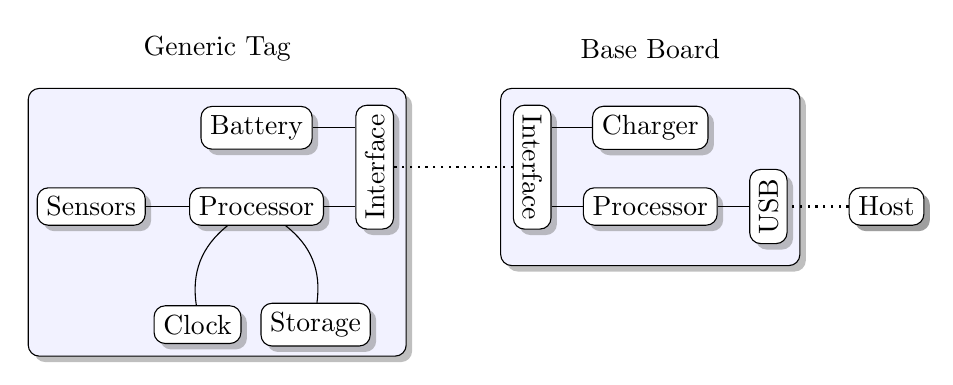
\begin{tikzpicture}[every node/.style={rounded corners,drop shadow}]

        \colorlet{lightgray}{black!5}


        %
        % Generic Tag
        %
        \filldraw[fill=blue!5, rounded corners, drop shadow] (-2.4,-2.4)
        rectangle (2.4,1);
        %
        %    nodes
        %
        \node (proc) at (0.5,-0.5)        [rectangle,draw,fill=white] {Processor};
        \node (bat) at  (0.5,0.5)        [rectangle,draw,fill=white]{Battery};
        \node (rtc) at  (-0.25,-2) [rectangle,draw,fill=white]{Clock};
        \node (mem) at  (1.25,-2)  [rectangle,draw,fill=white]{Storage};
        \node (sens) at (-1.6,-0.5)     [rectangle,draw,fill=white] {Sensors};
        \node (conn1) at (2,0)       [rectangle,draw,rotate=90,fill=white]
        {Interface};
        %
        %    edges
        %
        \path (rtc)   edge [bend left] (proc);
        \path (mem)   edge [bend right] (proc);
        \path (sens)  edge (proc);
        \path (proc) edge (proc -| conn1.north) ;
        \path (bat) edge (bat -| conn1.north);
        %
        %  Base board
        %
        \filldraw[fill=blue!5,rounded corners,drop shadow] (3.6,-1.25)
        rectangle (7.4,1);

        %
        %    nodes
        %
        \node (conn2) at (4,0) [rectangle,draw,rotate=-90,fill=white]
        {Interface};
        \node (chrg) at (5.5,0.5) [rectangle,draw,fill=white] {Charger};
        \node (proc2) at (5.5,-0.5) [rectangle,draw,fill=white] {Processor};
        \node (usb) at (7,-0.5) [rectangle,draw,rotate=90,fill=white] {USB};

        \node[rounded corners,rounded corners,drop shadow] (host) at (8.5,-0.5) [rectangle,draw,fill=white] {Host};
        %
        %    edges
        %

        \path (conn2)     edge [thick,dotted] (conn1);
        \path (chrg.west) edge (chrg -| conn2.north);
        \path (proc2)     edge (proc2 -| conn2.north);
        \path (usb)       edge (proc2);
        \path (host)      edge [thick,dotted] (usb);

        \begin{scope}[every node/.append style={reset preactions}]

                \node at (0,1.5) {Generic Tag};
                \node at (5.5,1.5) {Base Board};
        \end{scope}

        %  \draw[help lines] (-4,-2) grid (9,4);     

\end{tikzpicture}
\end{document}
